
	\subsection{\textit{Technical Analysis}}
	\label{tech-analysis}
	
	Untuk membuat sebuah aplikasi yang sukses, tentunya banyak sekali aspek yang harus diperhatikan. Selain kualitas aplikasi yang akan dibuat, juga ketahanannya terhadap perubahan karena \textit{e-commerce} adalah sesuatu yang sangat cepat berubah karena kompetitor yang sangat kompetitif dan dorongan tehnologi yang membuat efektifitas dan efisiensi menjadi lebih baik.\\
	
	\indent Dari aspek \textit{software engineering} sendiri, \textit{software engineering} dimaksudkan untuk menunjang/\textit{support} pengembangan \textit{software} daripada \textit{individual programming}. Hal ini mencakup: \begin{inlinelist}
		\item \textit{evolution}
		\item \textit{design}
		\item \textit{supporting program specification}
	\end{inlinelist} \cite{software-engineering}
	
	\begin{figure}[H]
		\centering
		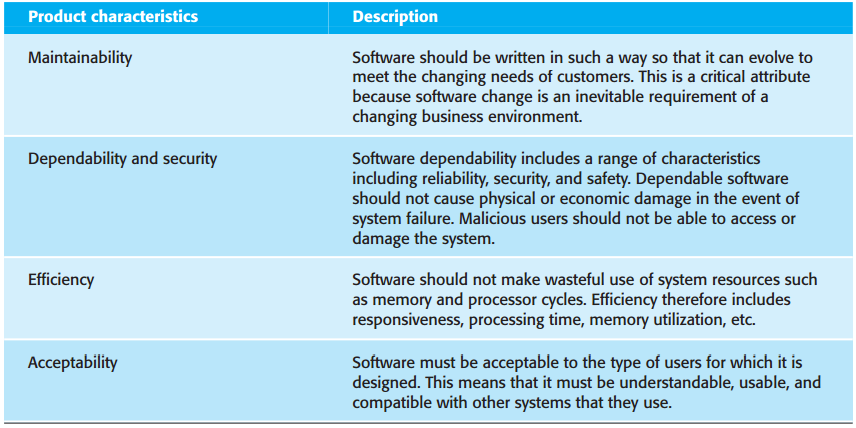
\includegraphics[width=\textwidth]{images/bab3/buku/essential-good-software.png}
		\caption{\textit{Essential attributes of good software}}
		\label{essential-software}
	\end{figure}
	
	\indent Berdasarkan kriteria tersebut, maka setiap poin perlu diperhatikan agar dapat mengembangkan sebuah aplikasi yang tidak hanya sukses, tapi juga bertahan dalam kompetisi. Dalam istilah bisnis, hal ini disebut dengan \textit{risk management \& planning}.
	

